\section{La integral definida}


\subsection{Notación ``Sigma''}


	La letra griega $\Sigma$ denota adición repetida:
	
	$$
	\sum_{i=a}^{b} f(i)=f(a)+f(a+1)+...+f(b),
	$$ siempre que $a\leq b.$



	\begin{problema}
		\label{ayr:exmp23.1}
		\begin{enumerate}
			\item $\sum_{j=1}^{5} j = 1+2+3+4+5 =15$ 
			\item $\sum_{i=0}^{3} \left( 2i+1 \right)=
			1+3+5+7$ 
			\item $\sum_{i=2}^{10} i^{2}=2^{2}+3^{2}+...+10^{2}$ 
			\item $\sum_{j=1}^{4}\cos(j\pi)=
			\cos\pi+ \cos 2\pi + \cos 3\pi +\cos 4\pi.$
		\end{enumerate}
		
	\end{problema}
	



	\subsection{Linealidad}
	\begin{proposicion}
		\label{suma:linealidad}
		\begin{align*}
			\sum_{i=a}^{b} cf(i)&=c \sum_{i=a}^{b} f(i)\\ 
			\sum_{i=a}^{b} f(i)+g(i)&= \sum_{i=a}^{b} f(i)
			+\sum_{i=a}^{b} g(i)
		\end{align*}
		
	\end{proposicion}
	


\subsection{Área bajo la curva}


	Sea $f$ una función tal que $f(x)\geq 0$ en el intervalo $[a,b].$
	



	\begin{figure}
		\centering
		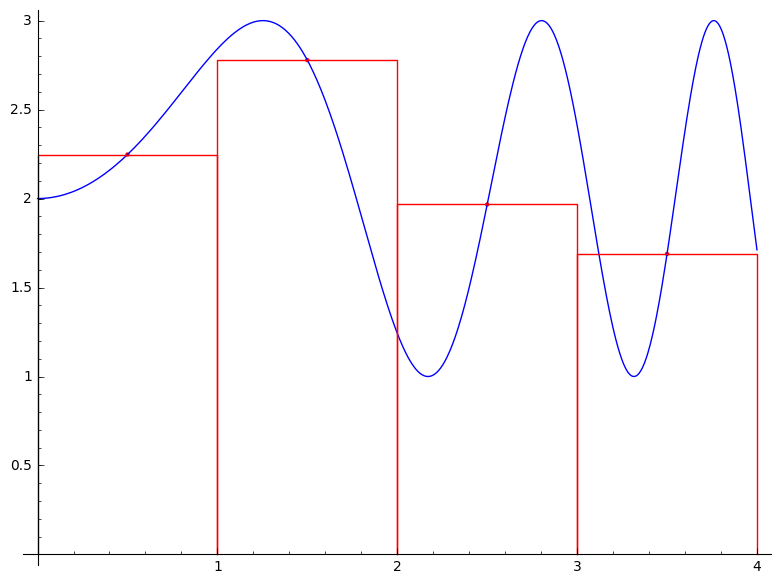
\includegraphics[height=5cm,keepaspectratio=true]{./calculo/tmp_h5b5ua.png}
		% tmp_h5b5ua.png: 0x0 pixel, 300dpi, 0.00x0.00 cm, bb=
		\caption{Aproximación de área bajo la curva}
		\label{fig:ayr:23.2}
	\end{figure}
	



	\begin{algoritmo}{Sumas de Riemman}
		\label{suma:riemann}
		\begin{enumerate}
			\item Dividimos el intervalo en $N$ subintervalos
			$$a=x_{0}<x_{1}<...<x_{N}=b.$$
			
			\item Definimos la longitud de cada intervalo $[x_{i-1},x_{i}]$ como $$\del x_{i}=x_{i}-x_{i-1}.$$
			
			\item El área bajo la curva definida por $f$ esta aproximada por
			$$\sum_{i=1}^{N} f(\xi_{i})\del x_{i},$$
			donde $\xi_{i}$ es un punto en el intervalo $[x_{i},x_{i+1}].$
		\end{enumerate}
	\end{algoritmo}



	Una manera más concreta de construir una suma de Riemman es \emph{fijando el tamaño del paso:}
	\begin{enumerate}
		\item Definimos $h=\dfrac{b-a}{N};$ 
		\item Escogemos $$\xi_{k}=a+kh, \, k=0,1,2,...,N;$$
		\item La suma de Riemann correspondiente será
		$$
		\sum_{k=1}^{N}f(\xi_{k})\cdot h=h\left( f(\xi_{1})+...+f(\xi_{N}) \right).
		$$
	\end{enumerate}
	



	Al fijar el tamaño del paso, hemos ocupado el extremo derecho de cada intervalo: $x_{k}=a+k*h,$ pero también podemos escoger por ejemplo:
	\begin{itemize}
		\item el extremo izquierdo:
		$$\xi_{k}=a+(k-1)\cdot h;$$ 
		\item o el punto medio de cada intervalo:
		$$\xi_{k}=a+\left( k-\dfrac{1}{2} \right) \cdot h;$$
	\end{itemize}
	




	Si en un intervalo $[a,b],$ $f(x)<0,$ entonces la suma anterior aproxima el área \emph{sobre la curva.}
	
	\begin{figure}
		\centering
		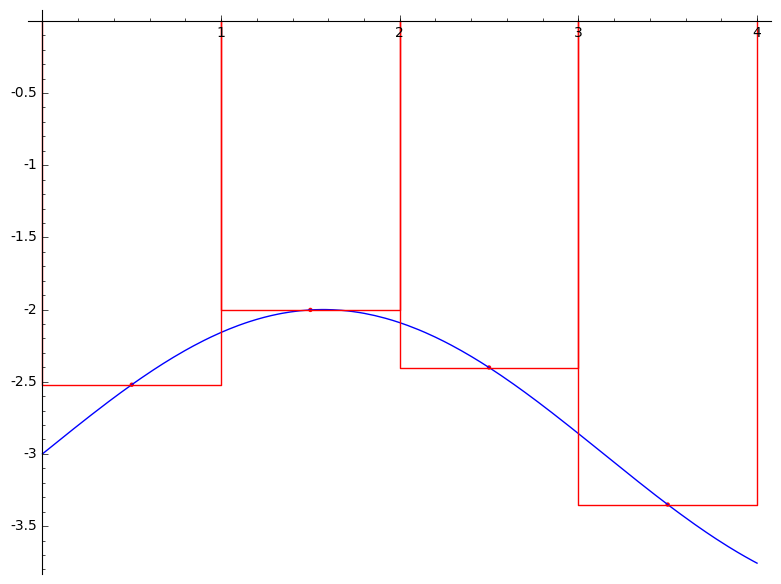
\includegraphics[height=5cm,keepaspectratio=true]{./calculo/tmp_pIdKIc.png}
		% tmp_h5b5ua.png: 0x0 pixel, 300dpi, 0.00x0.00 cm, bb=
		\caption{Aproximación de área bajo la curva}
		\label{fig:ayr:23.2}
	\end{figure}
	



	Por esta razón, cuando no distinguimos cuando $f(x)$ cambia de signo en un intervalo, hablamos del \emph{área con signo.}
	
	
	\begin{figure}
		\centering
		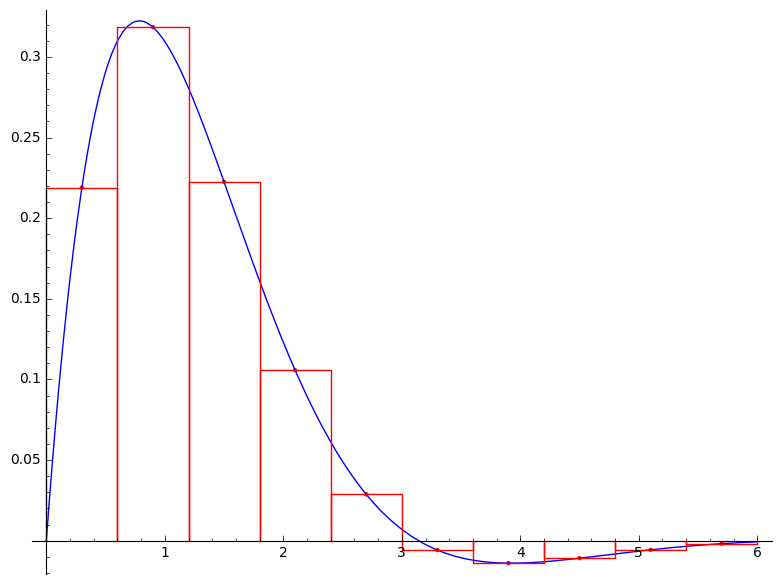
\includegraphics[height=5cm,keepaspectratio=true]{./calculo/tmp_pLz7nm.png}
		% tmp_h5b5ua.png: 0x0 pixel, 300dpi, 0.00x0.00 cm, bb=
		\caption{Aproximación de área bajo la curva}
		\label{fig:ayr:23.2}
	\end{figure}



	\begin{definicion}
		\begin{enumerate}
			\item   La integral definida de $f$ en el intervalo $[a,b]$ está dada por por
			$$
			\int_{a}^{b}f(x)dx=\lim_{N\to \infty}\left( \sum_{i=1}^{N} f(\xi_{i})\del x_{i} \right),
			$$ siempre y cuando el límite exista.
			
			
			\item  
			Si el límite existe, diremos que $f$ es integrable (en $[a,b]$).
			
			\item 
			La suma está definida como en el algoritmo \ref{suma:riemann} y se conoce como \emph{suma de Riemman.}
		\end{enumerate}
	\end{definicion}
	



	\begin{problema}
		Calcule
		$$\int_{1}^{5}1dx.$$
	\end{problema}
	



	\begin{problema}
		\label{ayr:exmp:23.3a}
		Calcule
		$$\int_{0}^{5}xdx.$$
	\end{problema}
	



	\begin{problema}
		\label{ayr:exmp:23.3b}
		Calcule
		$$\int_{1}^{5}xdx.$$
	\end{problema}
	



	\begin{proposicion}
		\begin{align}
			\label{ayr:23.2.1}
			\int_{a}^{b}1dx&=b-a\\ 
			\label{ayr:23.2.2}
			\int_{a}^{b}xdx&=\dfrac{b^{2}}{2}-\dfrac{a^{2}}{2}
		\end{align}
		
	\end{proposicion}
	



	\begin{problema}
		\label{exmp:evc:2.1}
		Aproxime la integral
		$$
		\int_{a}^{b} \dfrac{1}{\sqrt{2\pi}}e^{-\frac{1}{2}x^{2}}dx
		$$
		utilizando el algoritmo \ref{suma:riemann} fijando el tamaño del paso, con $a=-1, b=1, N=5$ y usando el extremo derecho de cada intervalo.
	\end{problema}



	\begin{problema}
		Aproxime la integral del ejemplo \ref{exmp:evc:2.1} cuando:
		\begin{enumerate}
			\item $a=0, b=3, N=4;$  
			\item $a=-2, b=2, N=8;$  
			\item $a=-3, b=3, N=16.$
		\end{enumerate}
		
	\end{problema}
	



\subsection{Propiedades de la Integral Definida}


	\subsection{Propiedades: Linealidad}
	\begin{align}
		\label{ayr:23.3}
		\int_{a}^{b} c f(x)dx&=c \int_{a}^{b}f(x)dx \\
		%   \label{ayr:23.4}
		%   \int_{a}^{b} -f(x)dx&=- \int_{a}^{b}f(x)dx\\		
		\label{ayr:23.5}
		\int_{a}^{b} \left( f(x)+g(x) \right)dx&= \int_{a}^{b}f(x)dx + \int_{a}^{b}g(x)dx
	\end{align}
	



	\subsection{Propiedades: Límites}
	\begin{align}
		\label{ayr:23.7}
		\int_{a}^{c}f(x)dx&=\int_{a}^{b}f(x)dx
		+\int_{b}^{c}f(x)dx\\		
		\label{ayr:23.7.i}
		\int_{a}^{a}f(x)dx&=0\\		
		\label{ayr:23.7.ii}
		\int_{a}^{b}f(x)dx&=-\int_{b}^{a}f(x)dx
	\end{align}
	


\subsection{Ejemplos Resueltos}


	\begin{problema}
		Supongamos que $f$ y $g$ son integrables en $[a,b].$ Demostrar que:
		\begin{enumerate}
			\item Si $f(x)\geq 0$ en $[a,b],$ entonces $\int_{a}^{b}f(x)dx\geq 0.$
			\item Si $f(x) \leq g(x)$ en $[a,b],$ entonces
			$$
			\int_{a}^{b}f(x)dx \leq \int_{a}^{b}g(x)dx.
			$$
			\item Si $m\leq f(x) \leq M$ para todo $x\in [a,b],$ entonces
			$$
			m\left( b-a \right) \leq \int_{a}^{b}f(x)dx
			\leq M\left( b-a \right).
			$$
		\end{enumerate}
	\end{problema}



%	\begin{problema}
%		%\label{ayr:solved:23.4}
%		Evalue $$\int_{0}^{1} x^{2} dx$$ a partir de la definición.
%	\end{problema}
	



	\begin{problema}
		\label{ayr:solved:23.5}
		Demuestre la fórmula
		$$
		\sum_{k=1}^{n}k=\dfrac{n\left( n+1 \right)}{2}.
		$$
	\end{problema}
	
